\documentclass{article}

% if you need to pass options to natbib, use, e.g.:
% \PassOptionsToPackage{numbers, compress}{natbib}
% before loading nips_2017
%
% to avoid loading the natbib package, add option nonatbib:
% \usepackage[nonatbib]{nips_2017}

\usepackage[final]{nips_2017}

% to compile a camera-ready version, add the [final] option, e.g.:
% \usepackage[final]{nips_2017}

\usepackage[utf8]{inputenc} % allow utf-8 input
\usepackage[T1]{fontenc}    % use 8-bit T1 fonts
\usepackage{hyperref}       % hyperlinks
\usepackage{url}            % simple URL typesetting
\usepackage{booktabs}       % professional-quality tables
\usepackage{amsfonts}       % blackboard math symbols
\usepackage{nicefrac}       % compact symbols for 1/2, etc.
\usepackage{microtype}      % microtypography
\usepackage{xspace}
\usepackage{graphicx}
\usepackage{caption}
\usepackage{subfig}
\usepackage[section]{placeins}

\title{Applying a Convolutional Neural Net to Street View House Numbers}

% The \author macro works with any number of authors. There are two
% commands used to separate the names and addresses of multiple
% authors: \And and \AND.
%
% Using \And between authors leaves it to LaTeX to determine where to
% break the lines. Using \AND forces a line break at that point. So,
% if LaTeX puts 3 of 4 authors names on the first line, and the last
% on the second line, try using \AND instead of \And before the third
% author name.

\author{
	Levi Butts\\
	CENG Undergraduate\\
	South Dakota School of Mines and Technology\\
	Rapid City, SD 57701 \\
	\texttt{Levi.Butts@mines.sdsmt.edu} \\
}

\newcommand{\MATLAB}{\textsc{Matlab}\xspace}

\begin{document}
	% \nipsfinalcopy is no longer used
	
	\maketitle
	
	\begin{abstract}
		Classifying text from natural images can be an incredibly difficult computer vision problem. When a learned feature based classification approach is used, positive results can clearly be seen. By applying a convolutional nueral network to the SVHN dataset we can classify numbers with surprising accuracy, approaching that of the previous benchmark set MNIST
	\end{abstract}
	
	\section{Introduction}
	
	Properly identifying text characters from photographs, in a timely manner, is one of the quintessential problems that machine learning programs aim to solve.  While the classification of controlled and restricted datasets is by and large a solved problem (i.e. recognizing handwritten digits, or characters in printed documents), performing similar tasks on images of natural scenes becomes much more difficult.  Natural phenomena: severe blur, distortion, illumination effects, etc. when coupled with the wide variation of font styles and display methods, are incredibly difficult to compensate for by hand.  A neural network operating on a learned feature-based classification method, such as image convolution, harbors plenty of potential to adequately handle this problem.   Utilizing a benchmark dataset captured from Google Street View images, which consists of over 600,000 digit images, this work will demonstrate the effectiveness of learned feature classification.
	
	Character recognition in images is a well studied, and well documented problem, with years of focused research performed by both academia and industry.  The MNIST digit dataset has been so thoroughly addressed that now it is used mainly as a jumping off point for machine learning beginners.  Any number of tutorials for the MNIST dataset can be found that produce near perfect accuracy with 'off-the-shelf' algorithms.  
	
	For this paper, the main focus will rest on taking the well-honed techniques used for the MNIST dataset and applying them to a restricted instance of scene-text recognition.  Namely the classification of house number signs in street level images from the Google Street View House Numbers (SVHN) dataset.  As stated previously, MNIST has been a valued standard for researchers seeking to improve their learning systems to compare against.  The SVHN dataset can be noted to have a style similar to MNIST, but SVHN comprises itself of data that comes from a significantly harder real world problem, and contains an order of magnitude more data than MNIST.
	
	To start, I will walk through details of the SVHN dataset in Section \ref{dt_set}, as well as the associated task of preparing and pre-processing required to properly interface the data with Tensorflow in Section \ref{pre-proc}.  Section \ref{model} will be an overview of the model design and the associated results will be discussed in Section \ref{results}.  All of this should adequately convey the power associated with feature based classification executed via a convolutional neural net.
	
	\section{Street View House Numbers (SVHN) Dataset}
	\label{dt_set}
		
	The SVHN dataset was compiled from a large number of Street View images from urban areas in various countries.  The house-numbers were extracted via a sliding window detector [3].  The dataset was then made available in two formats:
	
	\begin{itemize}
		\item Full Numbers - these are the original, variable resolution, color house-number images. Each image has character level bounding boxes and a transcription of the detected digits.
		
		\item Cropped Digits - these are formatted versions of the original images to resemble the MNIST set. Each image has been cropped and resized to be a fixed resolution of 32-by-32 pixels with the digit centered.
		  
	\end{itemize}
	
	As is explained in [3], the original collection of images for SVHN were compiled with the intent of using an end-to-end system that first detects the location of a house number in a larger image, then uses a detection stage to classify each digit (0 through 9).  For the purposes of this work I utilized the more controlled version of cropped images.  The cropped images were selected because the task of locating, identifying and processing the original images is a separate problem in and of itself.
	
	The dataset is divided into a total of three subsets:
	
	\begin{itemize}
		
		\item SVHN train - 73,257 digits for training
		\item SVHN test - 26,032 digits for testing
		\item SVHN extra - 531,131 additional, marginally less difficult samples, to use as extra training data
		
	\end{itemize}

	The first two subsets were obtained from a large number of Street View images. Even though SVHN-extra was generated in a similar manner, it is generally easier than SVHN-train and SVHN-test as a result of changes made to generate a dataset of such a large size.
	
	\begin{figure}
		\centering
		\subfloat[Examples of SVHN full images]{{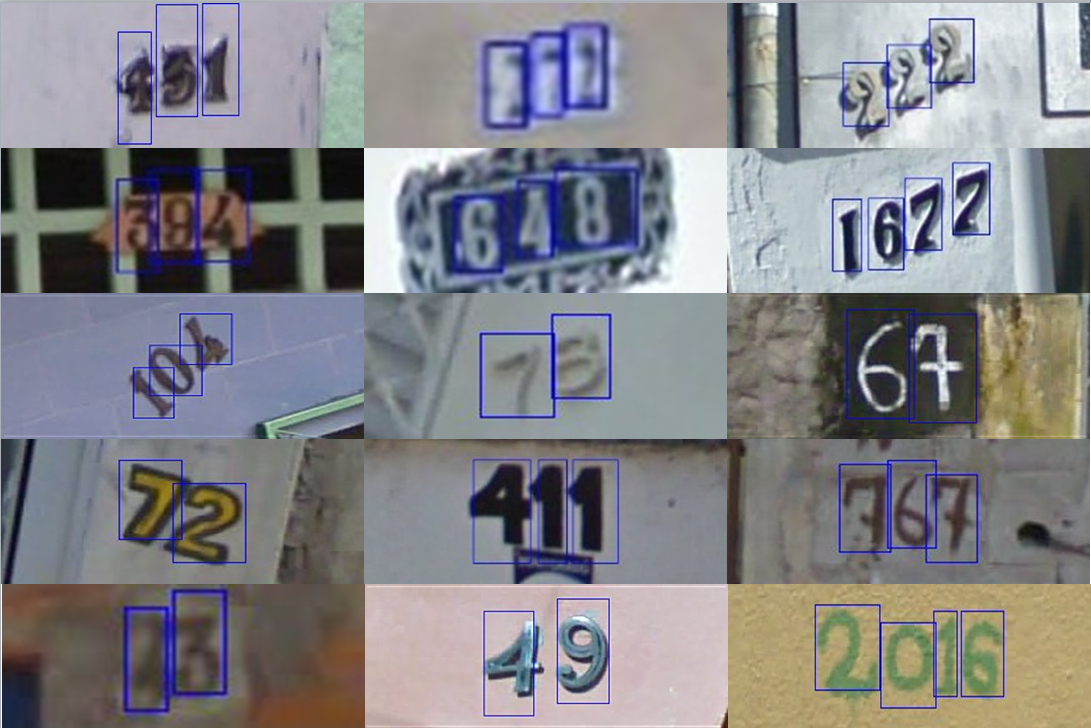
\includegraphics[width=6cm]{fullNum.png} }}%
		\qquad
		\subfloat[Examples of SVHN cropped images]{{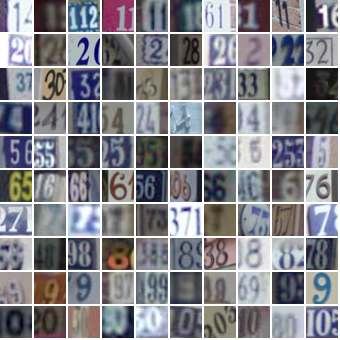
\includegraphics[width=6cm]{32x32eg.png} }}%
		\caption{Examples from SVHN Dataset}%
		\label{fig:examps}%
	\end{figure}
	
	\section{Data Pre-processing}
	\label{pre-proc}
		
	The SVHN dataset is available for free on the Internet and can be found at
	\begin{center}
		\url{http://ufldl.stanford.edu/housenumbers/}
	\end{center}
	where both the full-number and cropped-digit versions are available.
	
	The cropped-digits are saved as \MATLAB arrays inside of their respective .mat files. Properly interpreting the \MATLAB files was a substantial issue at the outset as they are parsed fairly differently from things like CSV, and IDX.  The solution for interpreting the .mat files was to convert them into .npy files consisting of numpy arrays. One common part of pre-processing is converting the labels int a vector of one-hot vectors; however, for this application it was decided not to do any one-hot encoding 
	to interface correctly with the Tensorflow loss function.

	\section{Model Design}
	\label{model}
	
	The model for this neural net is a relatively simple Tensorflow estimator.  The main structure of the model consists of two convolutional layers and two pooling layers which are alternated in order to pick out features and then reduce the size of the overall array.  The activation function used in each of the convolutional layers is ReLU.  After the last pooling layer there is a fully connected layer of 1024 nodes before the network finally produces its prediction.  During the final fully connected layer, A diagram of the overall network model can be found in Figure \ref{fig:model}
	
	\begin{figure}
		\centering
		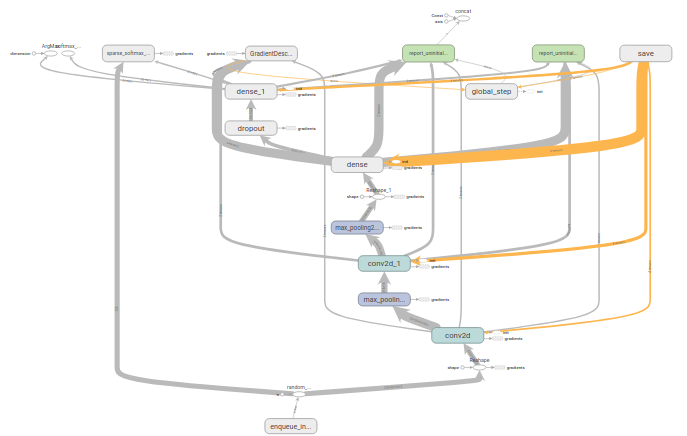
\includegraphics[width=0.7\linewidth]{Model.png}
		\captionsetup{width=0.7\linewidth}
		\caption{Graphical representation of the neural network's model}
		\label{fig:model}
	\end{figure}

	
	
	Early on, the design used three convolutional and pooling layers, it was later reduced to two to prevent unnecessary data loss. The first convolutional layer applies 25 filters each with a kernel size of 5-by-5 and implements zero-padding to ensure that the resulting output is the same dimensions as the input image. The second convolutional layer is very similar, the key difference being that it applies 50 filters as opposed to 25.
	
	The pooling layers utilize max pooling over a 2-by-2 filter meaning that after each pooling layer the output is approximately half of the size of the input. To evaluate the loss of network, after each iteration it uses Tensorflow's sparse softmax w/ cross entropy function. As mentioned earlier, the target labels are never one-hot encoded, which is because the loss function does not accept one-hot labels.
	
	\section{Results}
	\label{results}
	
	Presented here in \ref{fig:metrics} are the results of applying the model discussed above in Section \ref{model} to the SVHN dataset. 
	
	\begin{figure}[!htb]
		\centering
		\subfloat[Graph of Accuracy over time]{{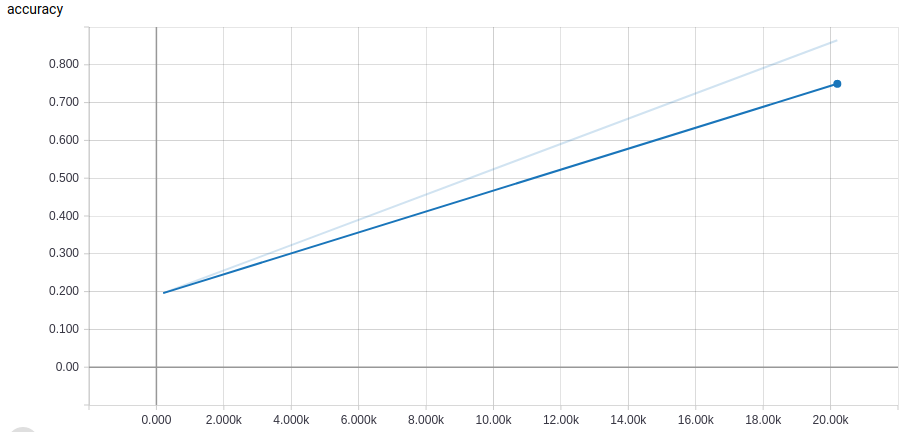
\includegraphics[width=6cm]{Accuracy.png} }}%
		\qquad
		\subfloat[Graph of loss over time]{{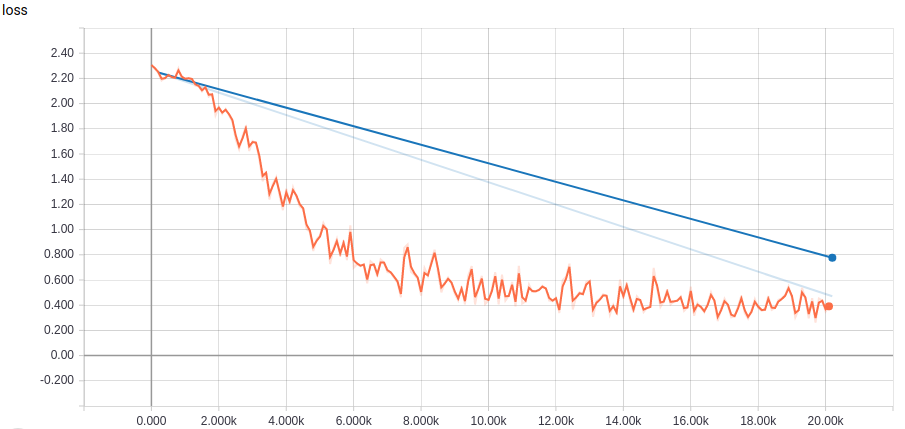
\includegraphics[width=6cm]{Loss.png} }}%
		\caption{Graphs of loss metrics for the network}%
		\label{fig:metrics}%
	\end{figure}
	
	
	In Figure \ref{fig:metrics} (b) the loss measured by our loss function takes a noticeable dip before leveling off around 0.4.  This behavior was not a surprise, and looks approximately as expected.
	
	As can be seen in Figure \ref{fig:metrics} (a) the overall accuracy of the network on the test set is roughly in the mid 80s.  When the accuracy is compared to that of a similar network applied to the MNIST dataset, (which averaged ~95\%) we can see that while the performance on our SVHN data isn't as good, it is  comparable in performance when the difference in difficulty between the two datasets is accounted for. Some possible changes that may be able to improve these results are tweaking of various hyper-parameters such as the learning rate, dropout rate, batch size, and the number of filters in each convolutional layer.
	
	\section{Conclusion}
	\label{conc}
	
	In this paper I have shown how applying a convolutional neural network to the SVHN dataset yields expected and promising resluts. With more tweaking of hyper-parameters and sequencing of convolutional and pooling layers, I believe that a network similar to this can reach MNIST levels of accuracy and performance. All of these things point to how feature based convolutional neural networks are incredibly adaptive and powerful without much cost of performance.
	
	
	\section*{References}
	

	\medskip
	
	\small
	
	[1] MNIST. http://yann.lecun.com/exdb/mnist/
	
	[2] SVHN. http://ufldl.stanford.edu/housenumbers/
	
	[3] Yuval Netzer, Tao Wang, Adam Coates, Alessandro Bissacco, Bo Wu,\ \& Andrew Y.Ng\ (2011) Reading Digits in Natural Images with Unsupervised Feature Learning. {\it NIPS Workshop on Deep Learning and Unsupervised Feature Learning 2011}
	
\end{document}